\begin{document}

\maketitle

\section{Sissejuhatus}
\begin{frame}[fragile]
  \frametitle{Eelmine kord}
  Peamine fookus IT valitsemisel
	\begin{itemize}
		\item IT valitsemine on naljakas pool-akadeemiline distsipliin. Keeruline kunst.
		\item Äriplaan mõjutab oluliselt arhitektuurseid ja tarkvaratehnilisi otsuseid
		\item Tehniline võlg võib juhtimatuna kergesti tagumikust hammustada
	\end{itemize}
\end{frame}

\begin{frame}[fragile]
  \frametitle{Täna kavas}
		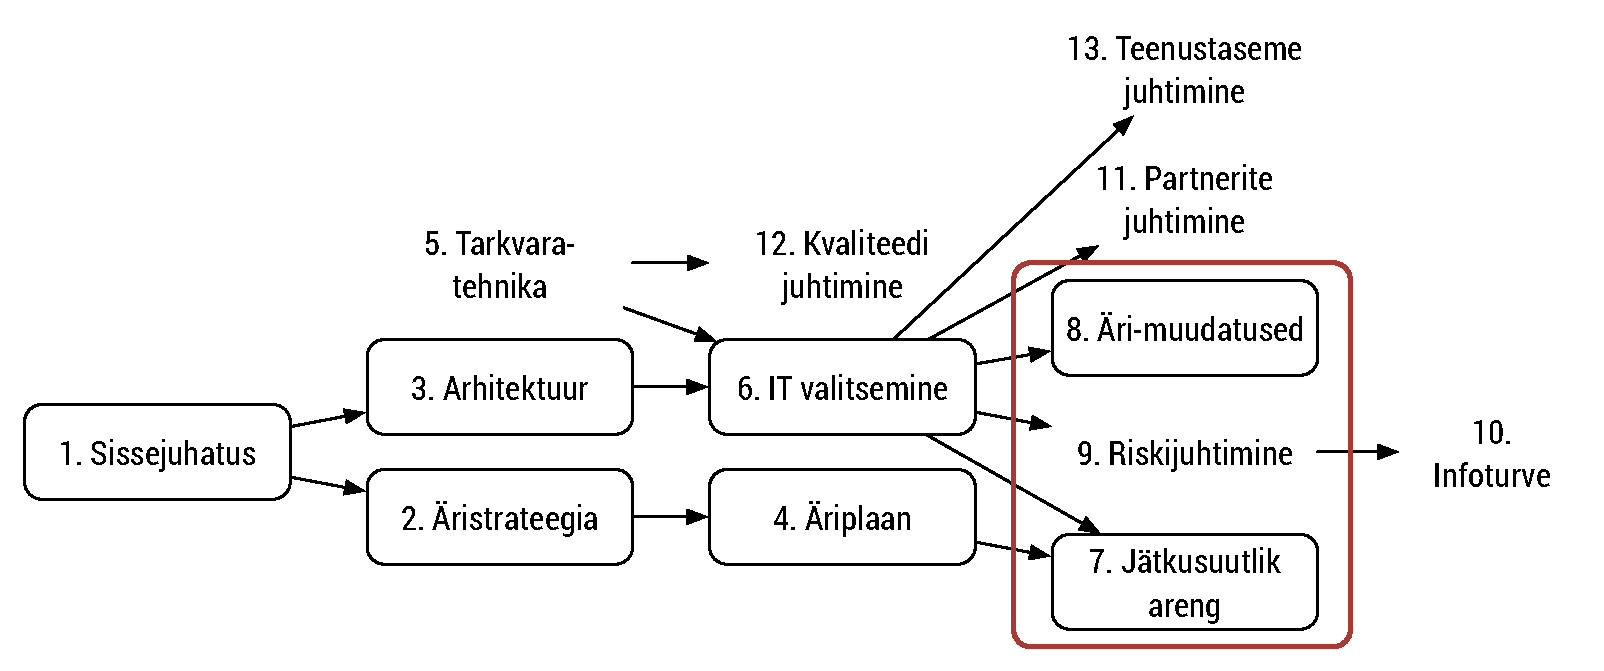
\includegraphics[width=\textwidth]{aine_struktuur_kolmas.pdf}
\end{frame}

\section{Jätkusuutlik areng}

%Arutelu koht
\begin{frame}[fragile]
  \frametitle{Arutelu koht}
		\begin{center}
			\textbf{1. küsimus}
		\end{center}
\end{frame}

%Arutelu koht
\begin{frame}[fragile]
  \frametitle{Arutelu koht}
		\begin{center}
			\textbf{2. küsimus}
		\end{center}
\end{frame}

\section{Ärimuudatused}
%Arutelu koht
\begin{frame}[fragile]
  \frametitle{Arutelu koht}
		\begin{center}
			\textbf{3. küsimus}
		\end{center}
\end{frame}

%Arutelu koht
\begin{frame}[fragile]
  \frametitle{Arutelu koht}
		\begin{center}
			\textbf{4. küsimus}
		\end{center}
\end{frame}

%Arutelu koht
\begin{frame}[fragile]
  \frametitle{Arutelu koht}
		\begin{center}
			\textbf{5. küsimus}
		\end{center}
\end{frame}

\section{Riskijuhtimine}
%Arutelu koht
\begin{frame}[fragile]
  \frametitle{Arutelu koht}
		\begin{center}
			\textbf{6. küsimus}
		\end{center}
\end{frame}


\section{Viited}

\begin{frame}[t,allowframebreaks,]
  	\bibliographystyle{plainnat}
	\bibliography{it_strateegia} 

\end{frame}

%\plain{Küsimusi?}
\begin{frame}[plain]
	\begin{center}Küsimusi?\end{center}
\end{frame}

\begin{frame}[fragile]
  \frametitle{Lahtised otsad ja ideed}
	\begin{itemize}
		\item Arthur Ganson Machine with Concrete kui näide muutuste põhjustest
		\item Keerukus ärimuutuste juures rääkida
		\item Iga loengu algusse slaid asukohaga skeemil
		\item \url{http://www.wired.com/2014/12/disappearing-business-of-design} näide ärimuutustest. Tehnilise kihi piirilt üles ja alla tagasi
		\item Nordea näide ärimuudatustega reageerimise juurde (oluline on kiirendus, mitte niivõrd kiirus)
	\end{itemize}
\end{frame}


\end{document}